%!TEX root = /Users/stevenmartell/Documents/CURRENT PROJECTS/iSCAM-trunk/docs/iSCAM-guide/overView.tex

\section{Running Examples} % (fold)
\label{sec:running_examples}
\begin{frame}
	\frametitle{Running examples}
	Examples in \texttt{iSCAM-trunk/examples}
	\begin{itemize}
		\item \texttt{Demo}
		\item \texttt{Hake}
	\end{itemize}
\end{frame}

\subsection{Demo Model} % (fold)
\label{sub:demo_model}


\begin{frame}
	\frametitle{Demo}
	\begin{itemize}
		\item The \texttt{Demo} directory is not present in the examples when you first checkout a copy of \iscam\ from the svn repository.
		\item To build the \texttt{Demo directory} cd to the examples directory and use \texttt{./makeproject Demo}
	\end{itemize}

\begin{figure}[htbp]
	\centering
		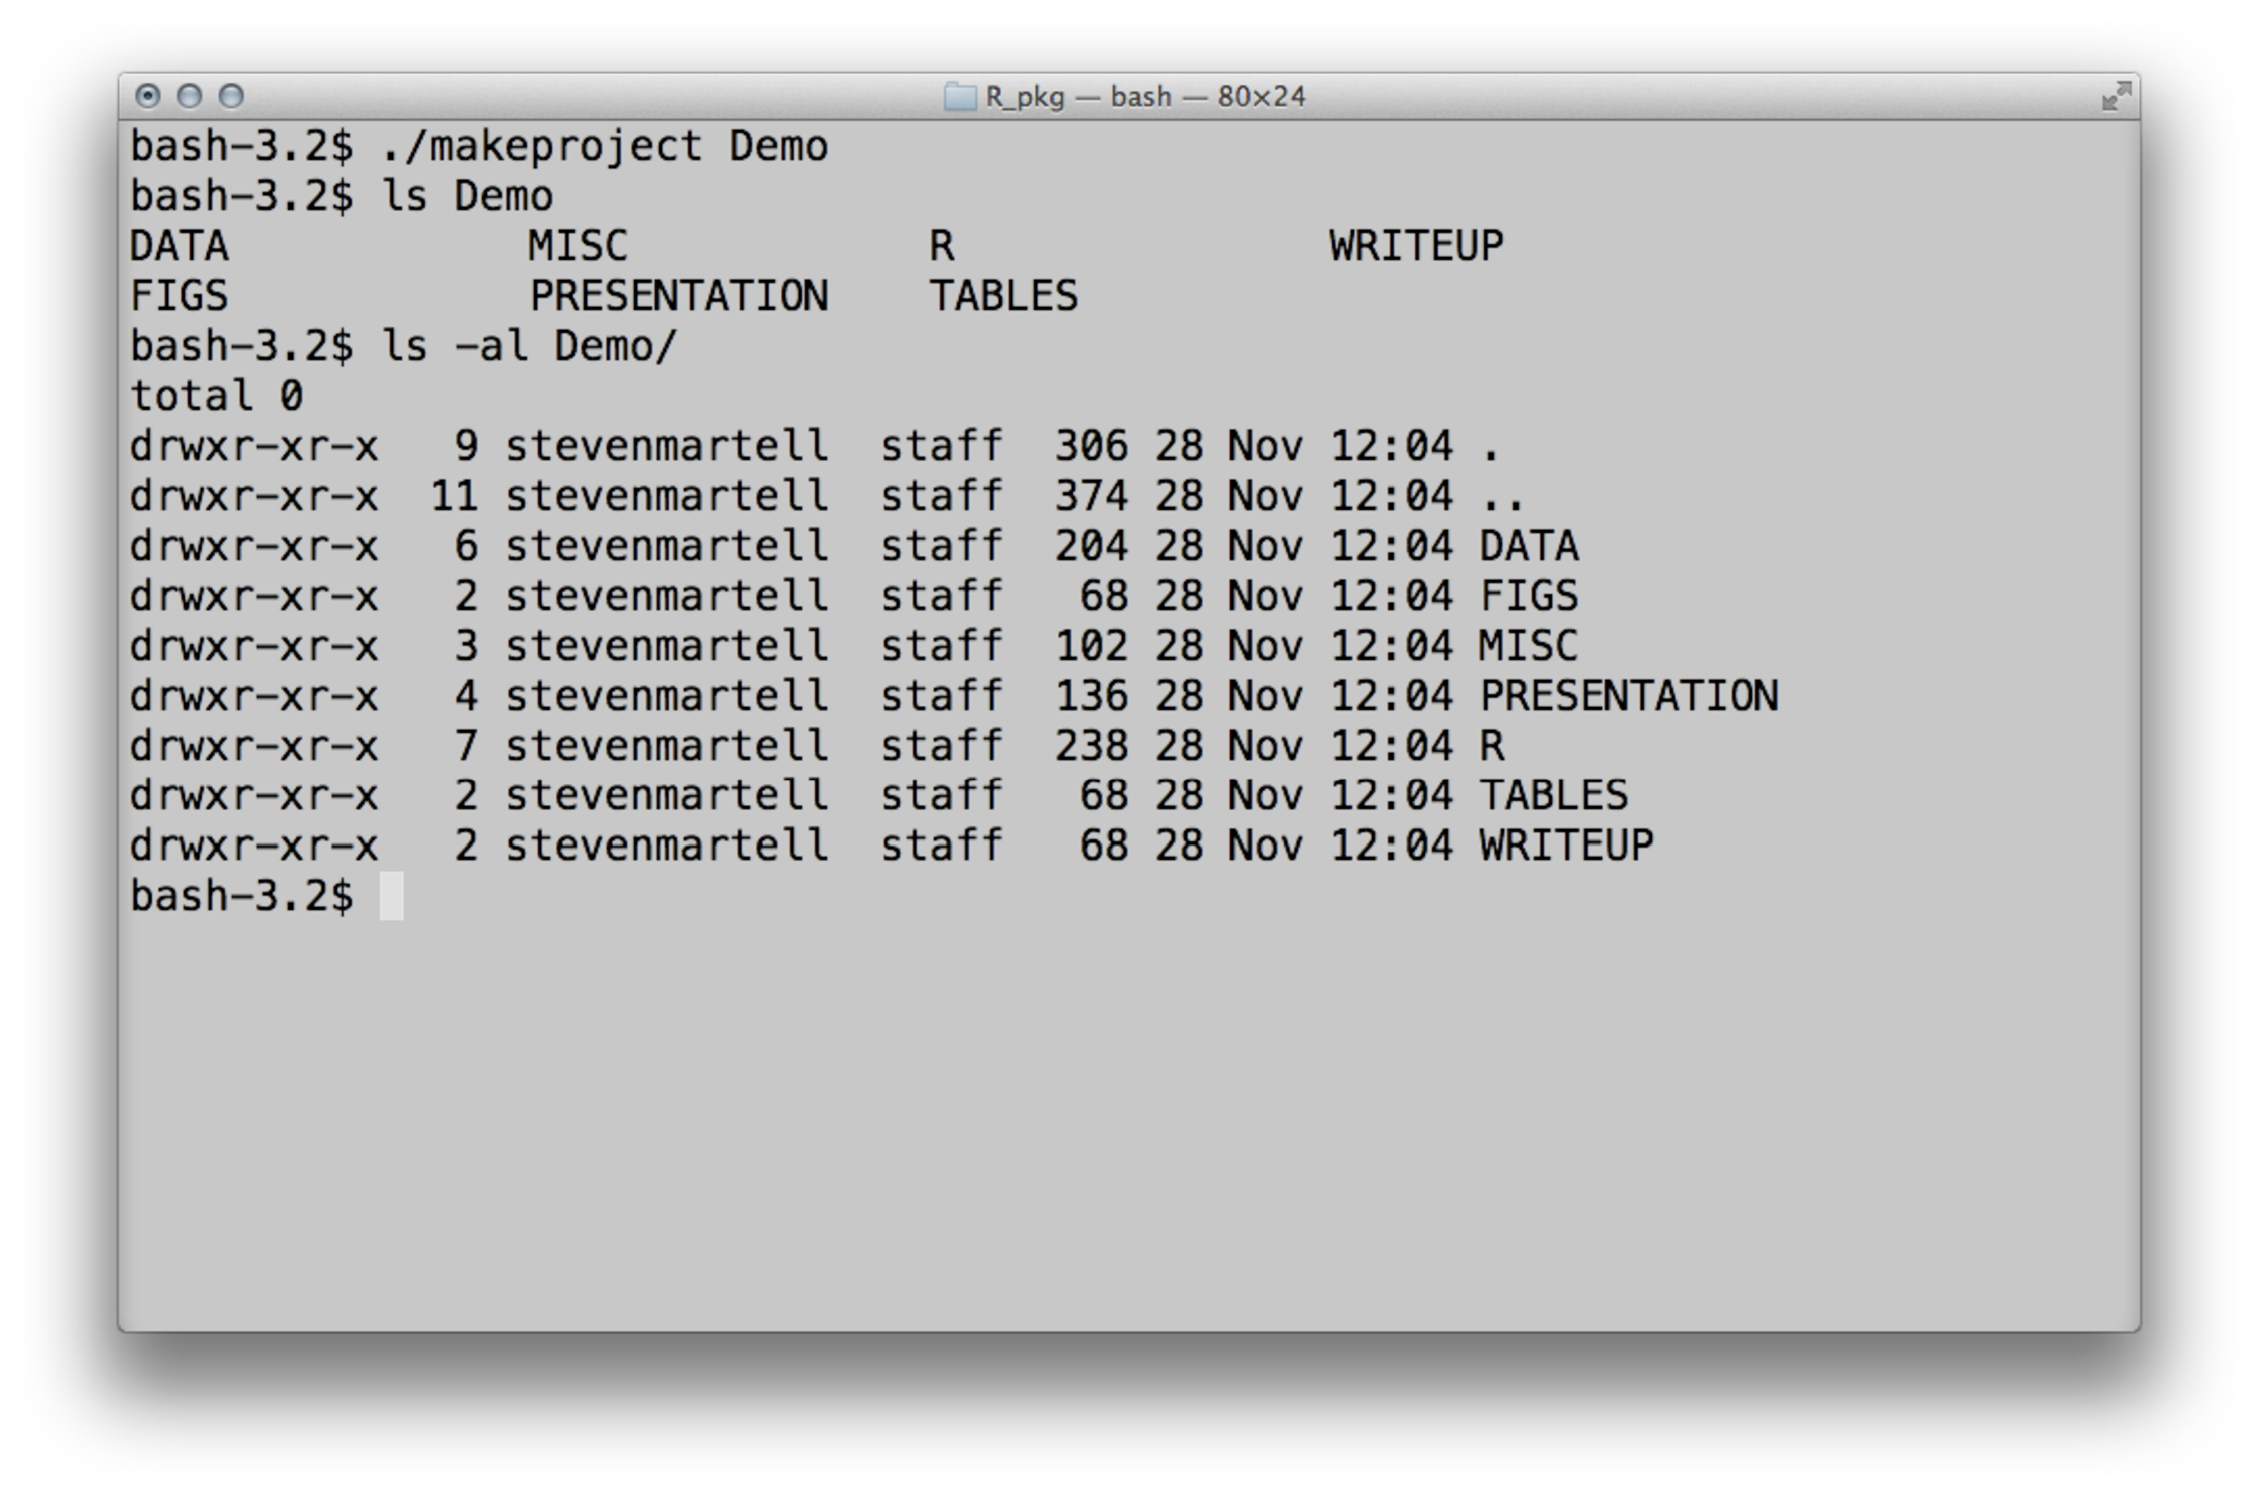
\includegraphics[height=1.75in]{screenCaptures/TermDemo.pdf}
	\caption{Using \texttt{makeproject} command to create \texttt{Demo}.}
	\label{fig:screenCaptures_TermDemo}
\end{figure}
\end{frame}

\begin{frame}
	\frametitle{Running the ADMB model in Demo}
	\begin{itemize}
		\item cd to the \texttt{examples/Demo/DATA} directory
		\item type \texttt{make} at the command line
	\end{itemize}
	\begin{figure}[htbp]
		\centering
			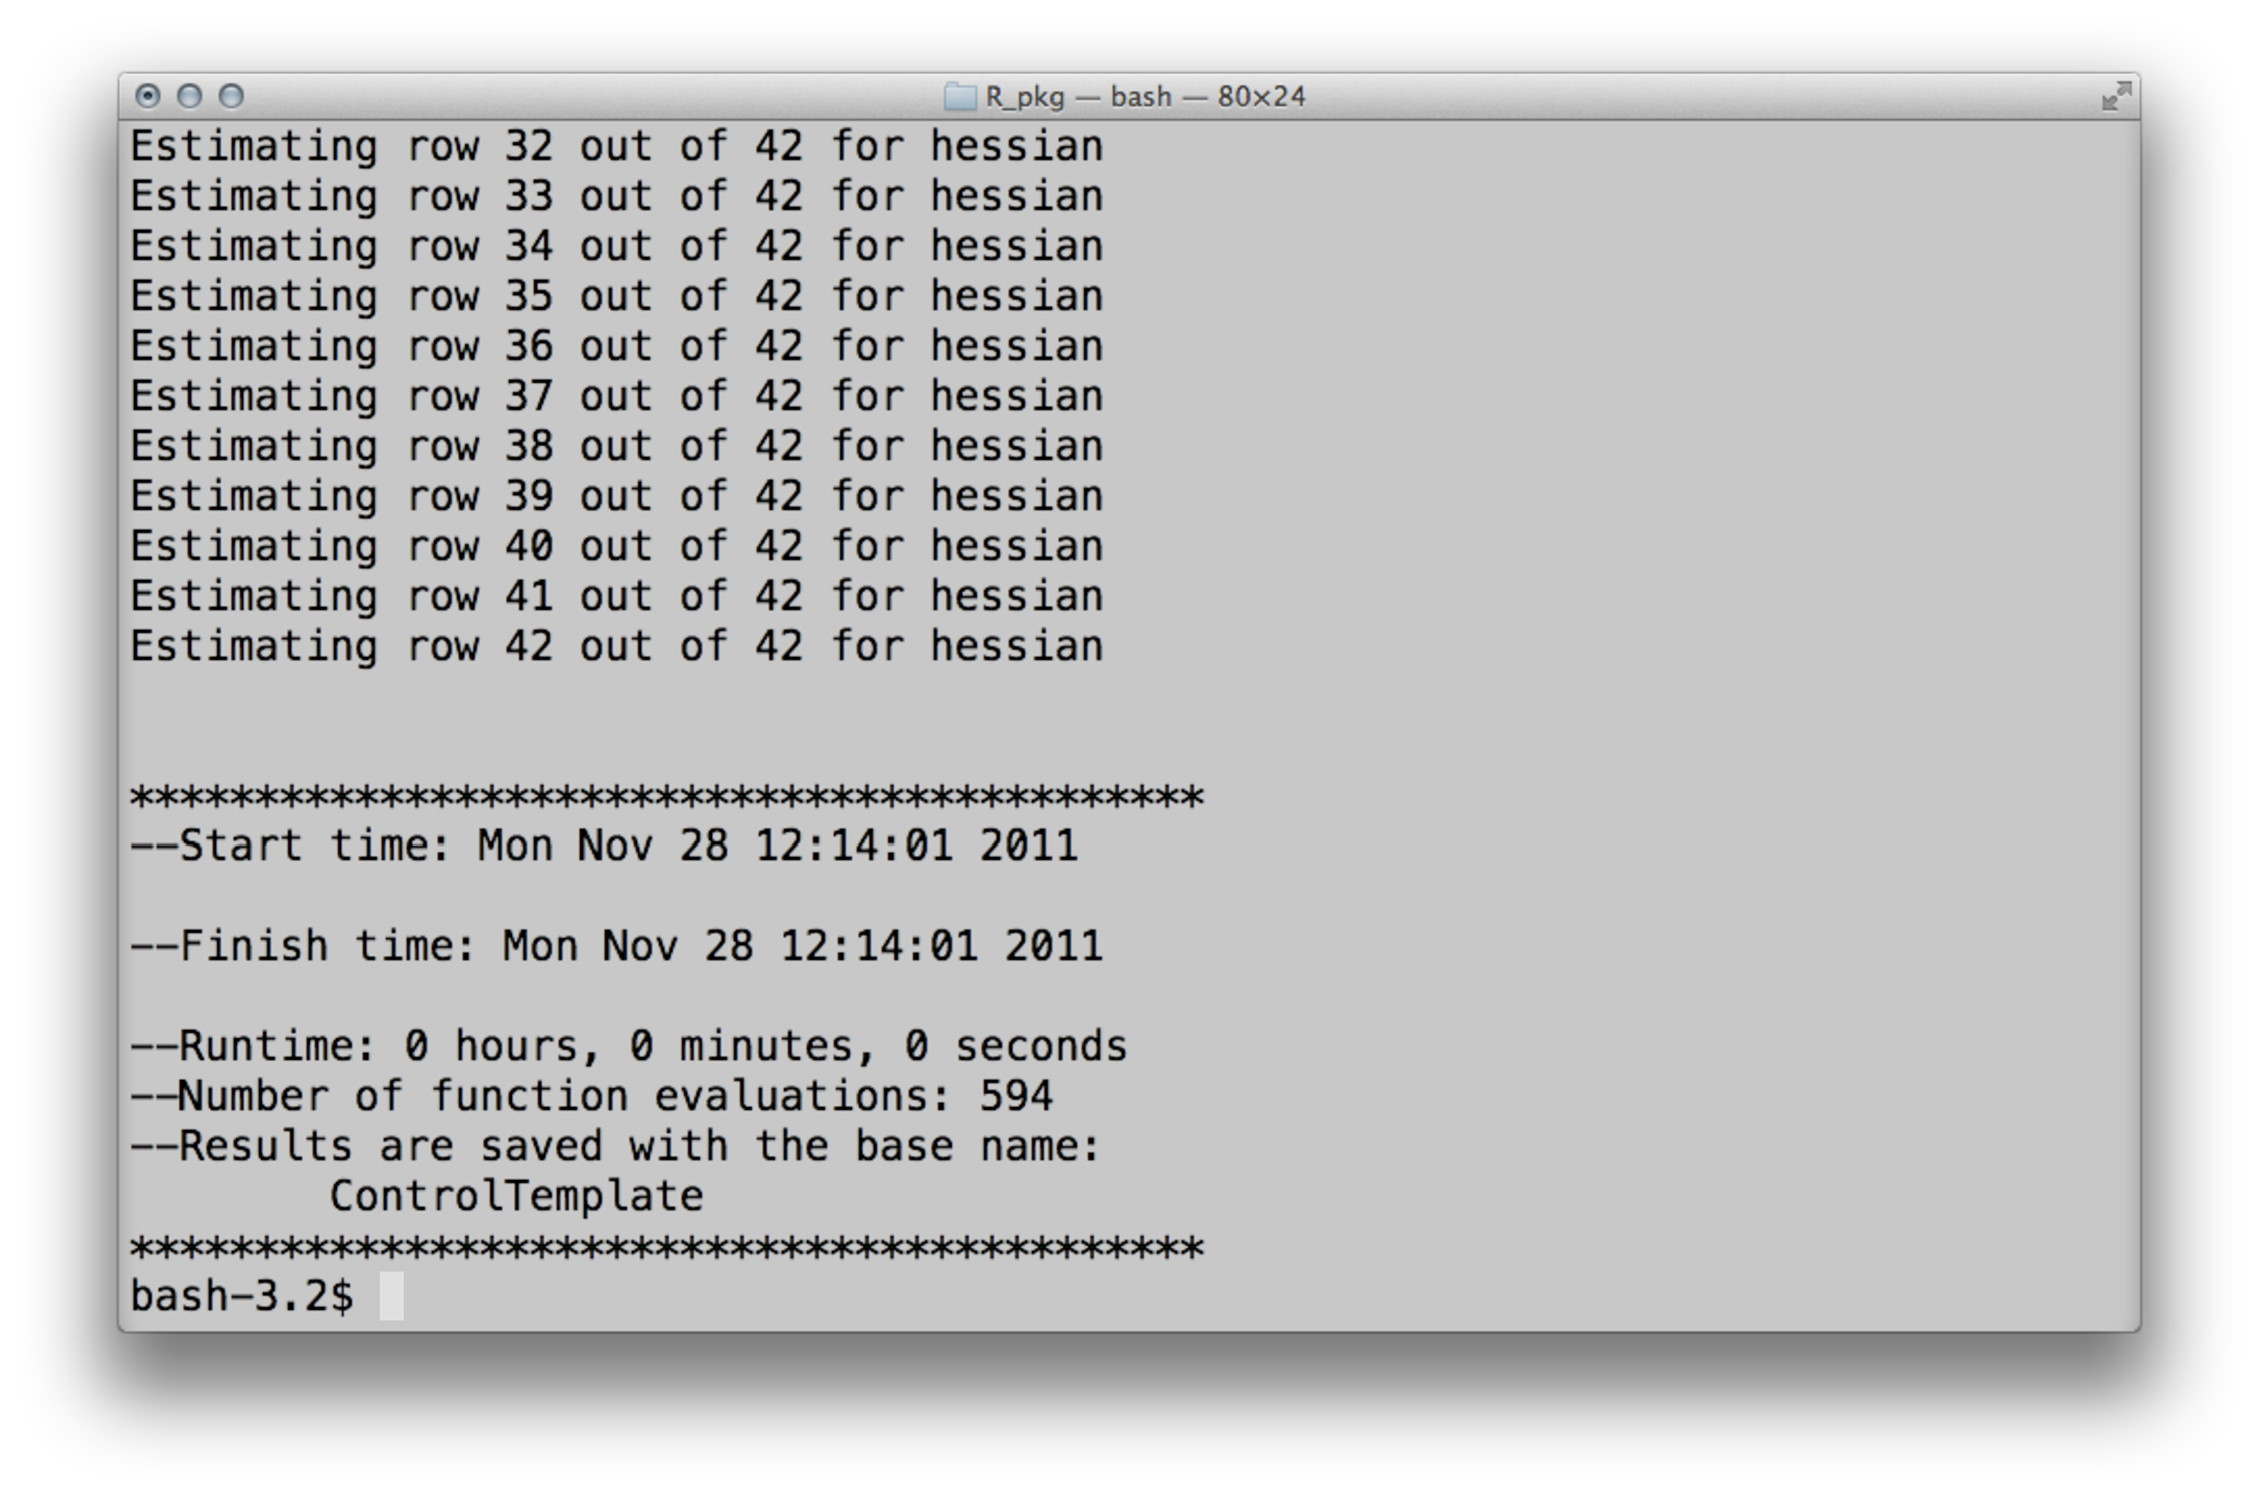
\includegraphics[height=1.75in]{screenCaptures/Term-catage.pdf}
		\caption{Terminal output after the Demo model has run}
		\label{fig:screenCaptures_Term-catage}
	\end{figure}
	
\end{frame}

\begin{frame}
	\frametitle{Using \texttt{guiView}}
	In the R directory, source the iSCAM.R file in R $>$guiView()
	\begin{figure}[htbp]
		\centering
			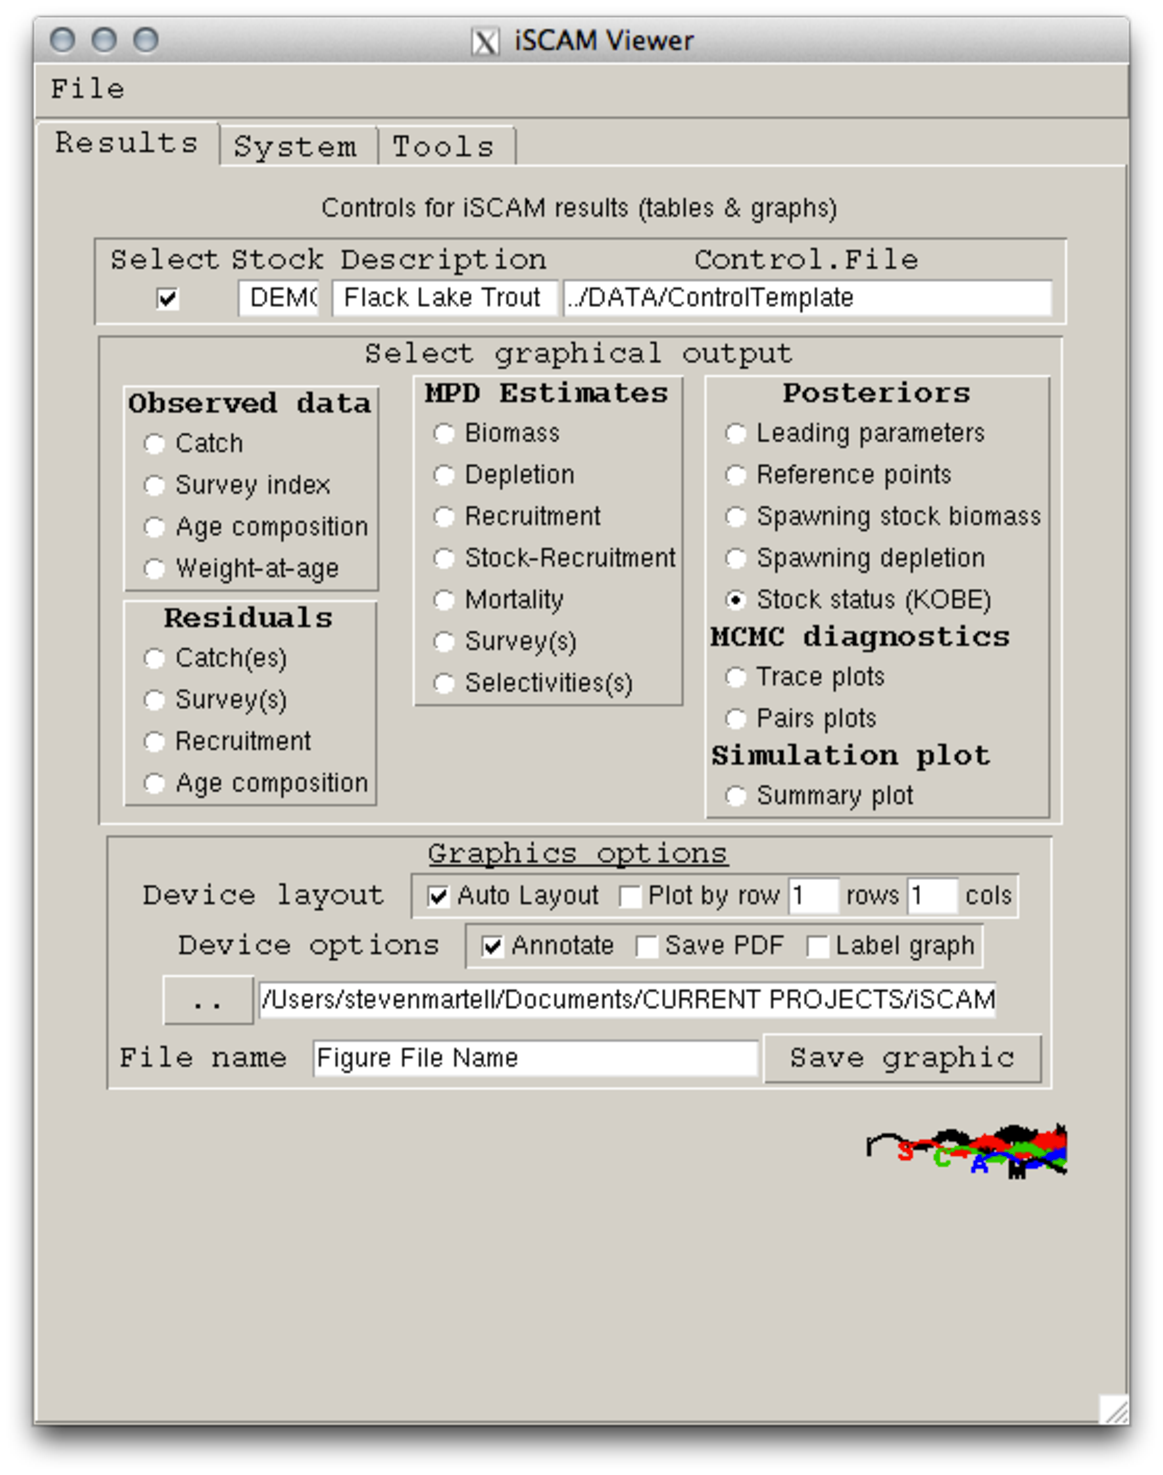
\includegraphics[height=2.5in]{screenCaptures/guiView.pdf}
		\caption{R gui for \iscam}
		\label{fig:screenCaptures_guiView}
	\end{figure}
	
\end{frame}
% subsection demo_model (end)
\subsection{Makefile} % (fold)
\label{sub:makefile}
\lstset{language=Pascal}
\begin{frame}[fragile,shrink=40]
	\frametitle{More on using \texttt{make}}
	\begin{code}
		
	
	\begin{lstlisting}
		## Makefile for running iscam
		## Targets: 
		##		all:   -copy executable and run the model with DAT & ARG
		##		run:   -copy executable and force a run
		##		mcmc:  -copy executable and run in mcmc mode and mceval
		##		retro: -copy executable and run  retrospective analysis
		EXEC=iscam
		prefix=../../../dist
		DAT=-ind RUN.dat
		CTL=ControlTemplate
		ARG=
		MCFLAG=-mcmc 10000 -mcsave 100 -nosdmcmc
		NR=4

		ifdef DEBUG
		  DIST=$(prefix)/debug/iscam
		else
		  DIST=$(prefix)/release/iscam
		endif
		\include{../../../scripts/ADMB_Makefile}
	\end{lstlisting}
	\end{code}
\end{frame}
% subsection makefile (end)
% section running_examples (end)